\documentclass{beamer}
\usepackage{ulem}
\usepackage{tikz}
\usepackage{booktabs}
 \usepackage{graphicx,threeparttable,caption}
\usetikzlibrary{shapes,snakes}
\usepackage[beamer,customcolors]{hf-tikz}
\usepackage{nicematrix}
\usepackage{xcolor}
\usepackage{makecell}
\usepackage{array}
\usepackage{csquotes}
\usepackage{csquotes}
\usepackage{minted}
\captionsetup{labelformat=empty,labelsep=none}

\graphicspath{ {./png/} }

\usetikzlibrary{
    arrows,
    arrows.meta,
    shapes,
    positioning,
    shadows,
    trees,
    calc
}

\tikzset{%
    >={Latex[width=2mm,length=2mm]},
    % Specifications for style of nodes:
    plain/.style = {},
    base/.style = {
        plain,
        rectangle, rounded corners, draw=black,
        minimum width=1cm, minimum height=1cm,
        text centered, font=\sffamily\tiny\bfseries,
        fill=white, align=center
    },
    app/.style = {base, ellipse},
    data/.style = {base, fill=gray!30},
    action/.style = {base, circle, fill=red!30},
    note/.style = {app, fill=yellow},
    hl/.style={
    set fill color=red!80!black!40,
    set border color=red!80!black
    }
}


\AtBeginSection[]{
  \begin{frame}
  \vfill
  \centering
  \begin{beamercolorbox}[sep=8pt,center,shadow=true,rounded=true]{title}
    \usebeamerfont{title}\insertsectionhead\par%
  \end{beamercolorbox}
  \vfill
  \end{frame}
}
\setbeamercolor{alerted text}{fg=orange}
%\usecolortheme[orchid]{structure}
\usetheme[hideothersubsections]{PaloAlto}
\makeatletter
\patchcmd{\csq@bquote@i}{{#6}}{{\emph{#6}}}{}{}
\makeatother
%\usecolortheme{orchid}
%\usefonttheme{professionalfonts}
\newcommand{\soutthick}[1]{%
   \textcolor{red}{
   \renewcommand{\ULthickness}{1pt}%
      \sout{#1}%
   \renewcommand{\ULthickness}{.4pt}% Resetting to ulem default
   }
}
\newcommand{\centered}[1]{\begin{tabular}{l} #1 \end{tabular}}
\setbeamertemplate{section in toc}[square]
\setbeamertemplate{subsection in toc}[square]
\setbeamertemplate{section in sidebar}[shaded]
\setbeamertemplate{items}[square]
\setbeamercovered{transparent} 

\title[]{Computational Social Science: An Introduction to Data Science}
\subtitle{Projects}
\author[]{Mikołaj Biesaga\\ \small{\color{blue}{\href{mailto:m.biesaga@uw.edu.pl}{m.biesaga@uw.edu.pl}}}}
\institute{
\includegraphics[width = 4 cm]{uw.png}}
\date{\today}
\begin{document}
\begin{frame}
   \titlepage
\end{frame}

\part[Example]{Example}
\frame{\partpage}

\begin{frame}
    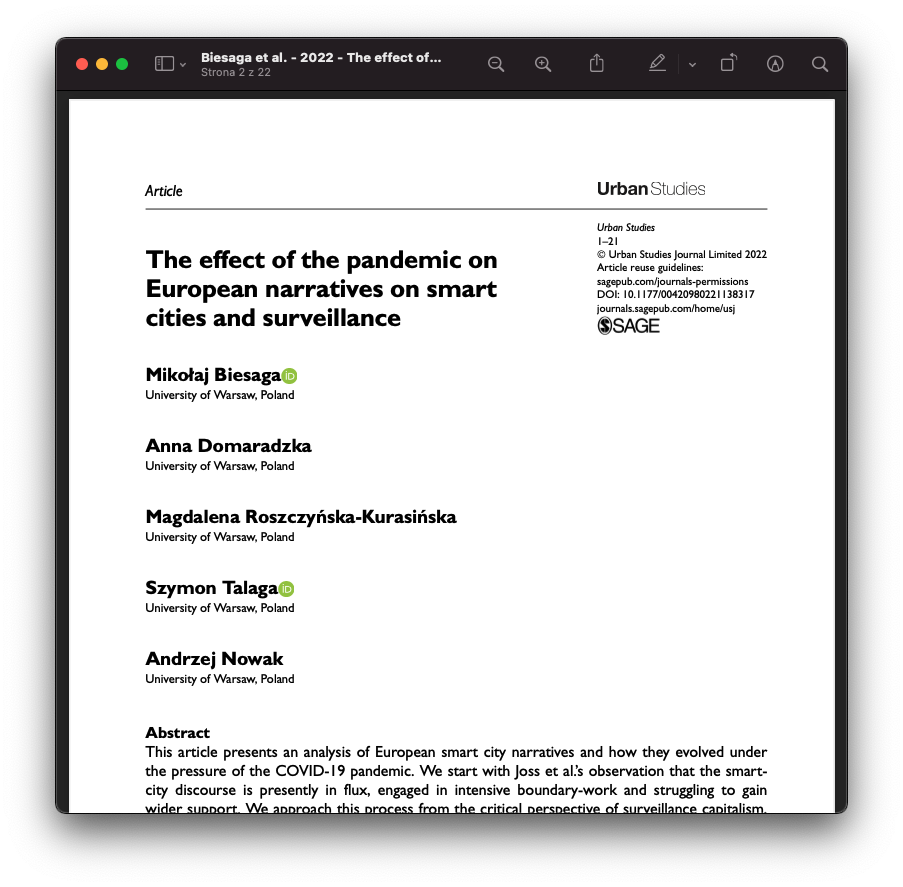
\includegraphics[width = \textwidth]{us.png}
\end{frame}



\section{Introduction}
\begin{frame}
   \frametitle{Introduction}
   \only<1>{
      \begin{itemize}
         \small
         \item The use of \alert{sensors and ICT tools} in an effort to
         ''flatten the curve''. The increase of smart city technologies
         implementation as a response to the COVID-19 pandemic.
         \item Growing \alert{virtualization and digitalization} of the urban
         realm as a response to the emerging challenges in terms of
         technological and social public space. 
         \item The \alert{danger} is that we develop technology \alert{without}
         reflecting on the \alert{normative, behavioral, and ethical} aspects of
         the new environment it produces for \alert{individuals}.
         \item \alert{Improving} the city for everyone begins with ensuring
         \alert{technology enhances democracy}, which means translating the
         right to the city idea into smart city solutions and policymaking that
         recognizes a citizen’s right to mobilize technology to shape urban
         spaces and to benefit from urban data.
      \end{itemize}
   }
   \only<2>{
      \framesubtitle{Motivation/Research problem}
      \begin{block}{}
         We wanted to observe whether the \alert{COVID-19 pandemic changed} the
         narrative on the transition of European cities into smart cities and
         consequently \alert{accelerated the implementation of smart city
         technologies}. We expected that the intensity of the changes shifted
         the existing narrative towards threats that excessive data collection
         on citizens poses.
      \end{block}
   }
\end{frame}
\section{Method}
\begin{frame}
   \frametitle{Method}
   \framesubtitle{Analysis Strategy}
   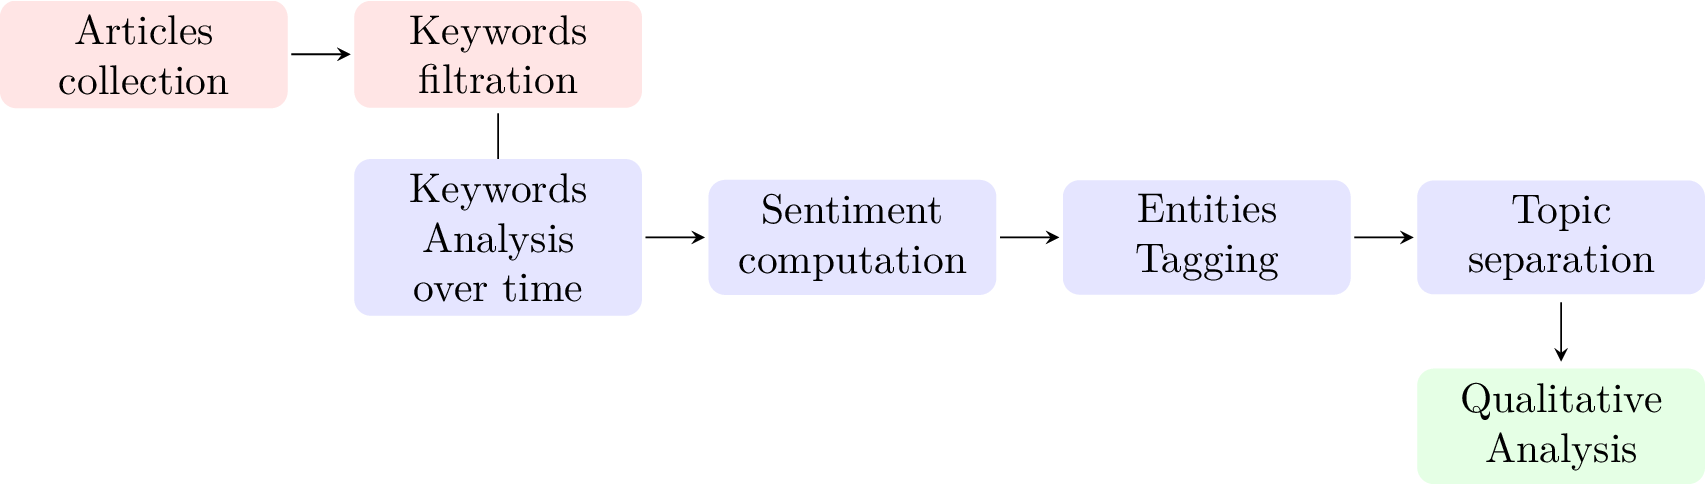
\includegraphics[width = \textwidth]{scheme.png}
\end{frame}
\begin{frame}[t]
   \frametitle{Method}
   \only<1-2>{
      \framesubtitle{Articles collection \& Keywords filtration}
      %\setbeamercolor{block body}{bg=red!10,fg=black}
      \begin{enumerate}[1]
         \item<1-> Sources selection
         %\item<2-> Facebook posts collection
         \item<2> Articles collection
      \end{enumerate}
      \only<1>{
         \begin{block}
            \centering
            \scriptsize
            \setcellgapes{4pt}\makegapedcells
            \begin{tabular}{|p{.35\textwidth}|>{\centering}p{.27\textwidth}|>{\centering\arraybackslash}p{.23\textwidth}|}
                \hline
                \bfseries{Source name}& \bfseries{Facebook Followers} & \bfseries{Facebook Likes} \\
                \hline
                \hline
                POLITICO Europe & $164\ 065$ & $156\ 291$ \\
                \hline
                Euronews English & $2\ 182\ 331$ & $2\ 107\ 895$ \\
                \hline
                EUobserver & $139\ 582$ & $139\ 194$ \\
                \hline
                EURACTIV & $45\ 453$ & $42\ 790$ \\
                \hline
                The Parliament Magazine & $5\ 222$ & $4\ 850$ \\
                \hline
            \end{tabular}
      \end{block}
      }
%      \only<2>{
%         \begin{figure}
%            \centering
%            
\includegraphics{sotrender_black.png}
%         \end{figure}
%      }
      \only<2>{
         \begin{block}
            \centering
            \scriptsize
            \setcellgapes{4pt}\makegapedcells
            \begin{tabular}{|p{.35\textwidth}|>{\centering}p{.17\textwidth}|>{\centering}p{.17\textwidth}|>{\centering\arraybackslash}p{.13\textwidth}|}
                \hline
                \bfseries{Source name}& \bfseries{Complete corpus} & \bfseries{Reduced corpus} & \bfseries{Final corpus} \\
                \hline
                \hline
                POLITICO Europe & $12\ 660$ & $161$ & $48$\\
                \hline
                Euronews English & $35\ 172$ & $205$ & $43$\\
                \hline
                EUobserver & $10\ 924$ & $62$ & $22$\\
                \hline
                EURACTIV & $9\ 745$ & $156$ & $48$\\
                \hline
                The Parliament Magazine & $1\ 656$ & $41$ & $23$\\
                \hline
            \end{tabular}
      \end{block}
      }
   }
   \only<3>{
      \framesubtitle{Keywords Analysis over time}
      \begin{center}
        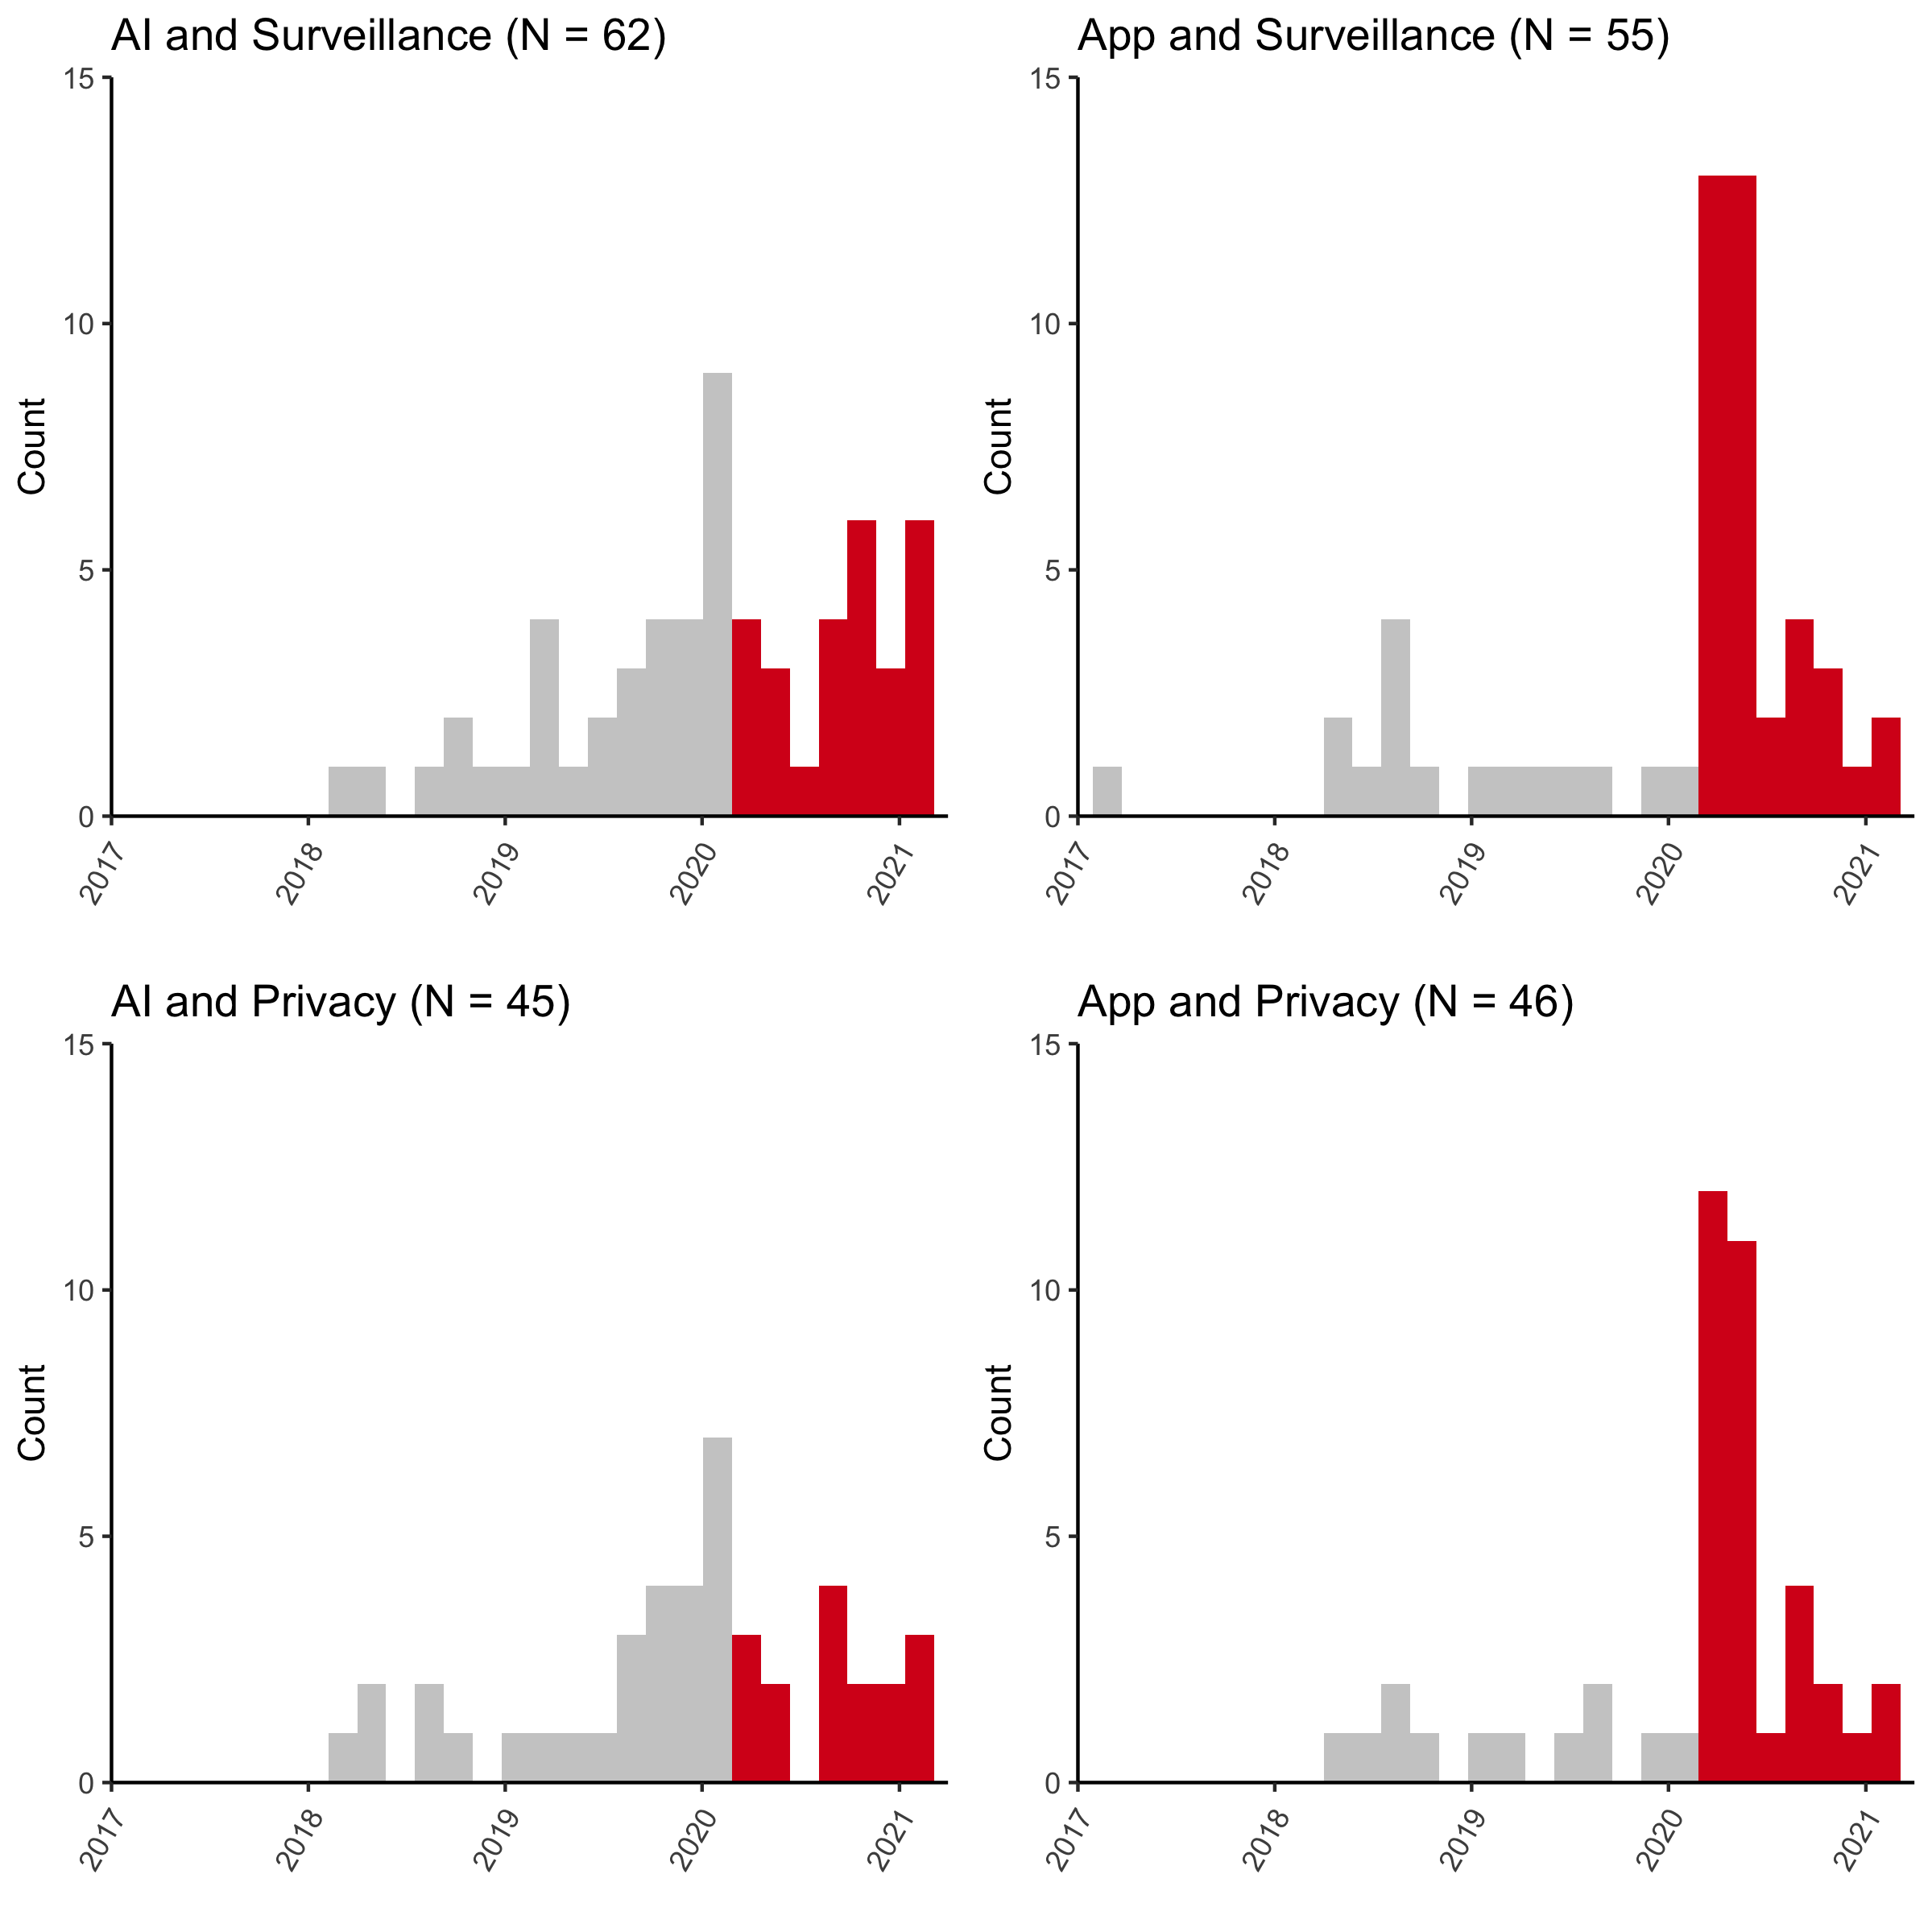
\includegraphics[width = .7\textwidth]{panel_plot.png}
      \end{center}
   }
   \only<4-6>{
      \framesubtitle{Sentiment Computation \& Entities Tagging \& Topic separation}
      \begin{itemize}
         \item<4-> Automatic Sentiment Computation\only<4>{\footnote[1]{Hutto C., Gilbert, E. (2014). Vader: A parsimonious rule-based model for sentiment analysis of social media text. \textit{Proceedings of the International AAAI Conference on Web and Social Media}, 8(1).}}
         \item<5-> Entities Tagging\only<5>{\footnote[2]{Honnibal M., Montani, I., Van Landeghem, S. (2020) spaCy: Industrial-strength Natural Language Processing in Python. Software.}}
         \item<6-> Topic Separation -- Latent Dirichlet Allocation\only<6>{\footnote[3]{Blei, D.M., Ng, A.Y., Jordan M.I. (2003). Latent dirchlet allocation. \textit{Journal of machine Learning research}, 3:993--1022.}}
      \end{itemize}
%      \only<4>{
%         \begin{equation*}
%            Sentiment = compuond \times (1 - Neutral)
%         \end{equation*}
%      }
      \only<5>{
         \centering
         
\includegraphics[width = .4\textwidth]{spacy.png}
      }
      \only<6>{
         \begin{block}
            \centering
            \scriptsize
            \centering
            \setcellgapes{2pt}\makegapedcells
            \begin{tabular}{|p{.2\textwidth}|>{\centering\arraybackslash}p{.30\textwidth}|}
                \hline
                \bfseries{Topic} & \bfseries{Number of Articles} \\
                \hline
                \hline
                Topic 1 & $82$ \\
                \hline
                Topic 2 & $13$ \\
                \hline
                Topic 3 & $38$ \\
                \hline
                Topic 4 & $4$ \\
                \hline
                Topic 5 & $28$ \\
                \hline
                Topic 6 & $5$ \\
                \hline
                Topic 7 & $14$ \\
                \hline
            \end{tabular}
         \end{block} 
      }
   }
\end{frame}
\section{Quantitative Analysis}
\begin{frame}
   \frametitle{Quantitative Analysis}
   \setbeamertemplate{caption}{\raggedright\insertcaption\par}
   \only<1-2>{
      \framesubtitle{Topic 1: AI and facial recognition.}
      \only<1>{
         \begin{figure}
            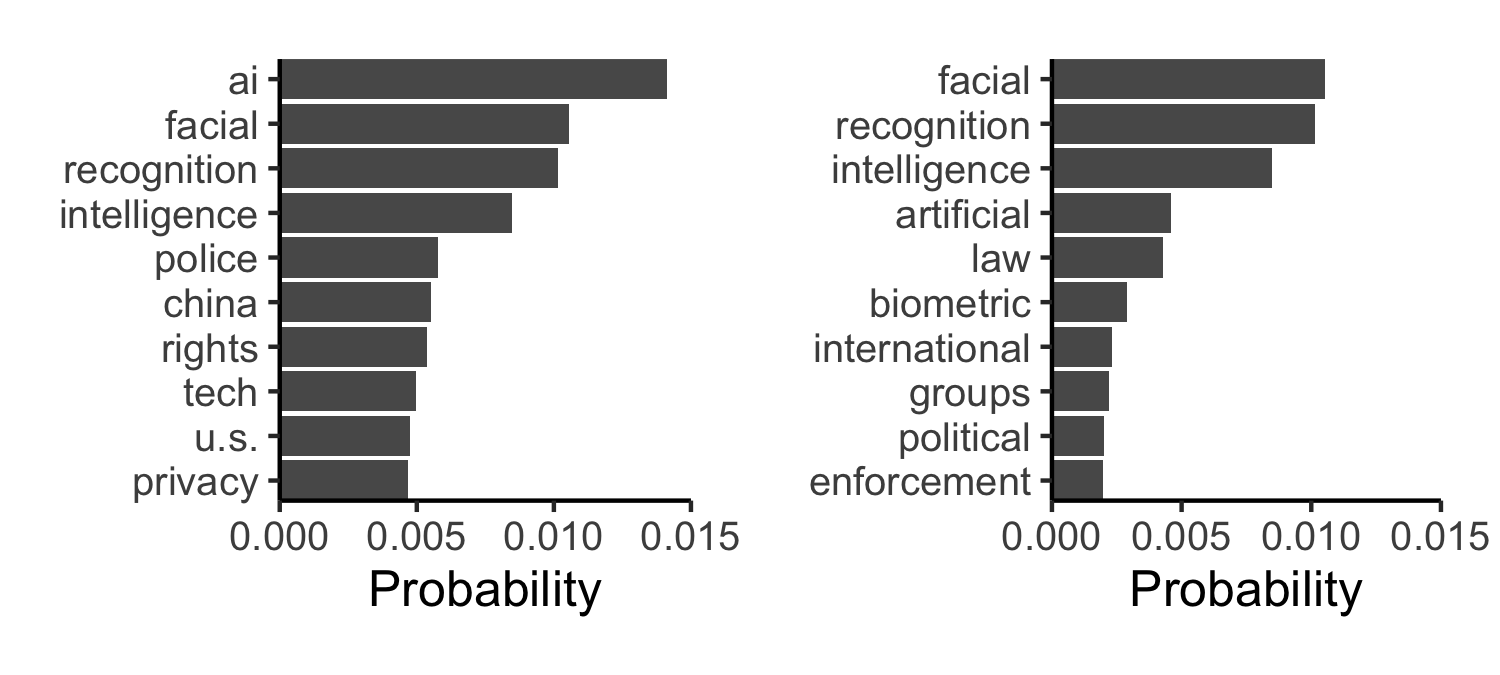
\includegraphics[width = \textwidth]{topic1.png}
            \caption{\alert{The left panel} shows the most probable words while \alert{the right panel} depicts probablity of the words that are unique only for the topic.}
         \end{figure}
      }
      \only<2>{
         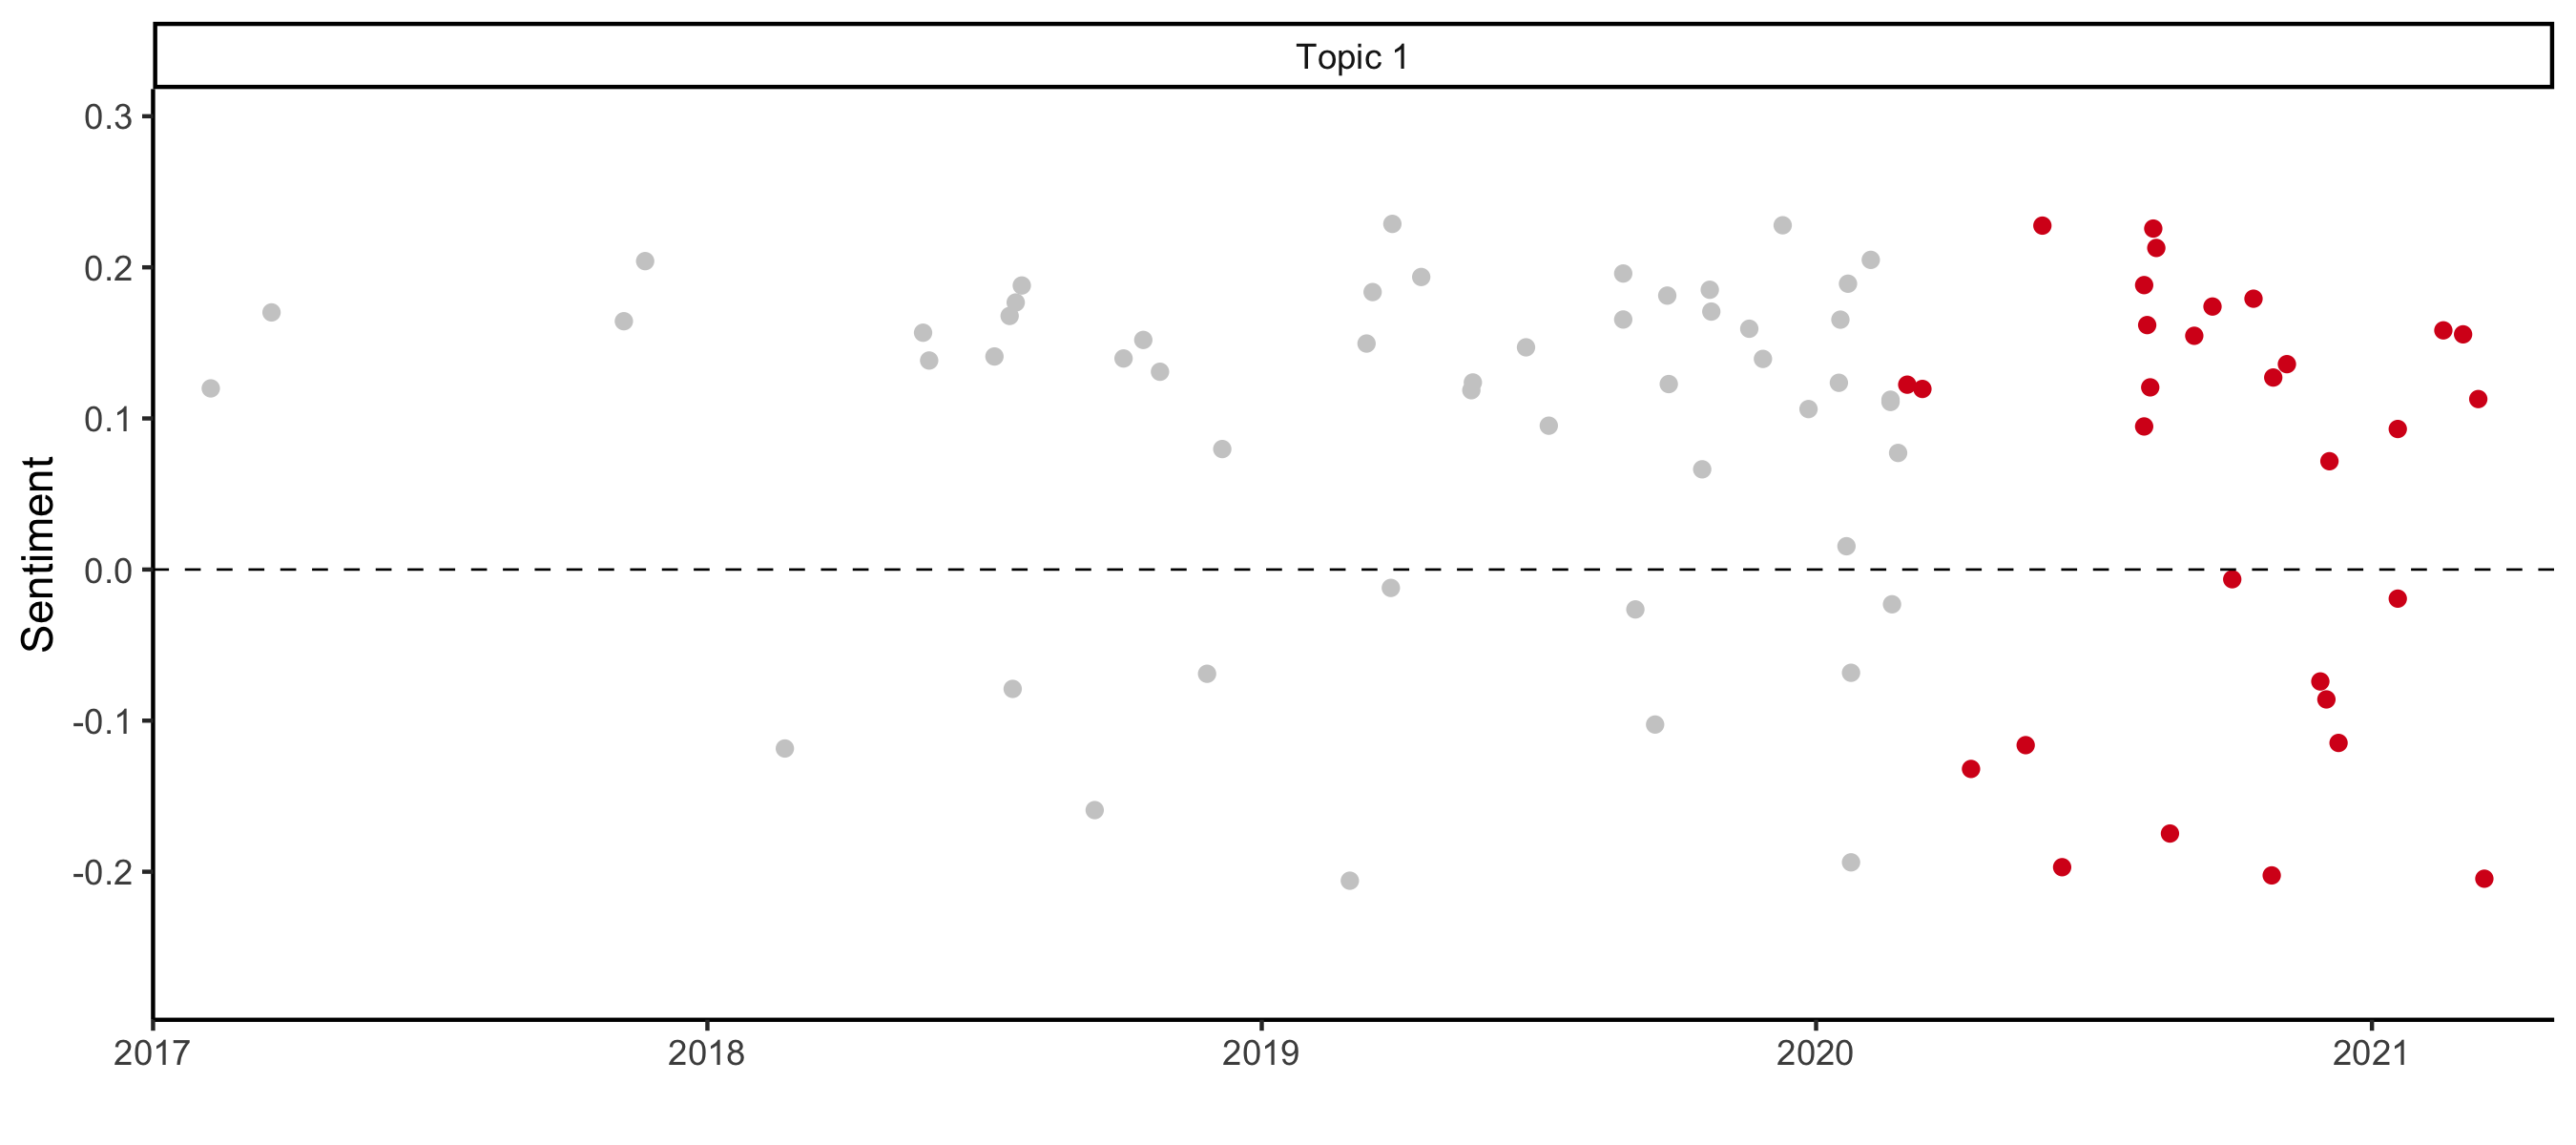
\includegraphics[width = \textwidth]{topic1red.png}
      }
   }
   \only<3-4>{
      \framesubtitle{Topic 2: Smart technologies to fight the climate emergency}
      \only<3>{
         \begin{figure}
            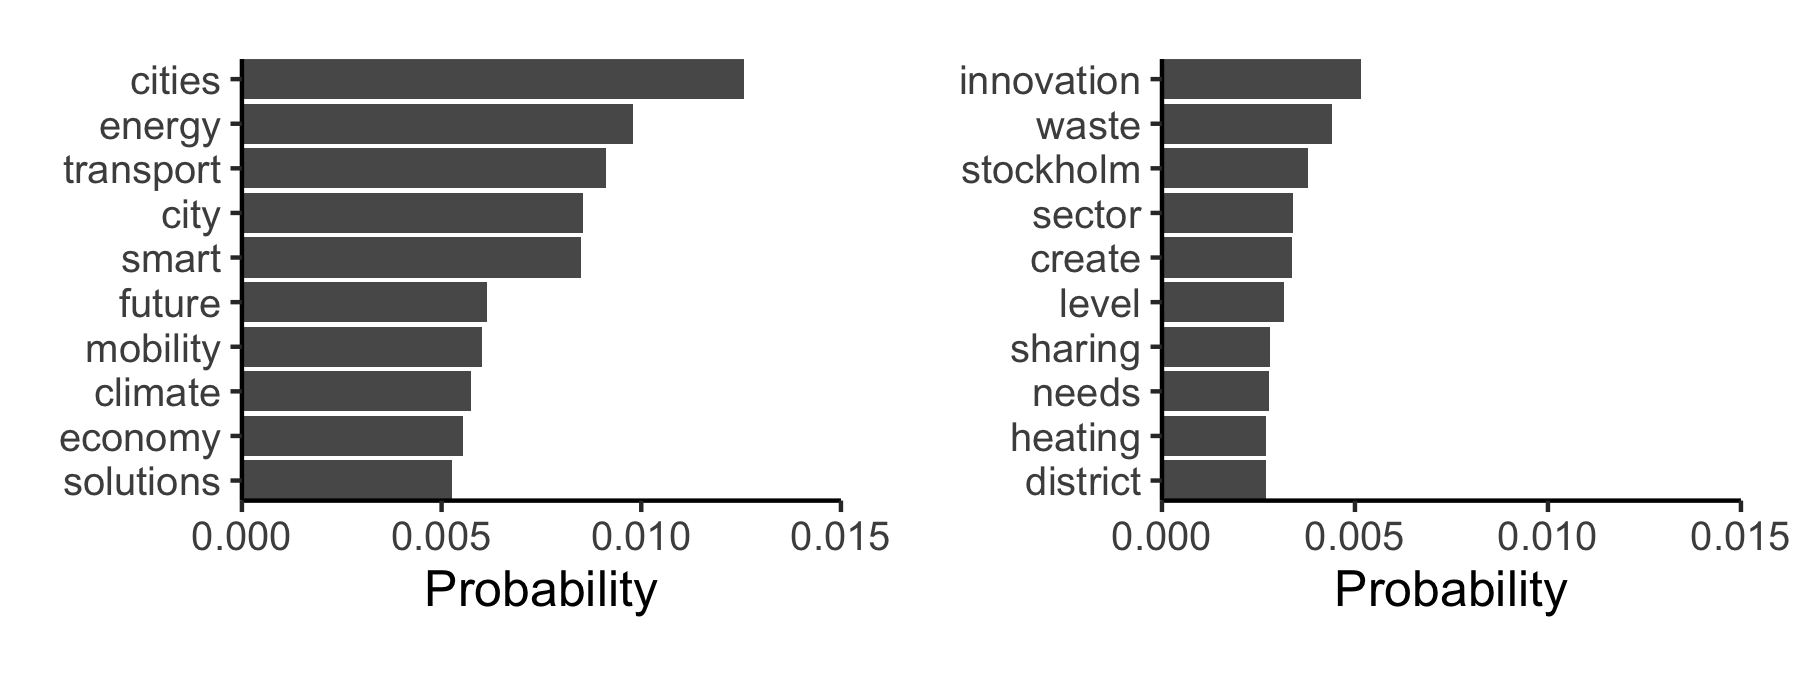
\includegraphics[width = \textwidth]{topic2.png}
            \caption{\alert{The left panel} shows the most probable words while \alert{the right panel} depicts probablity of the words that are unique only for the topic.}
         \end{figure}
      }
      \only<4>{
         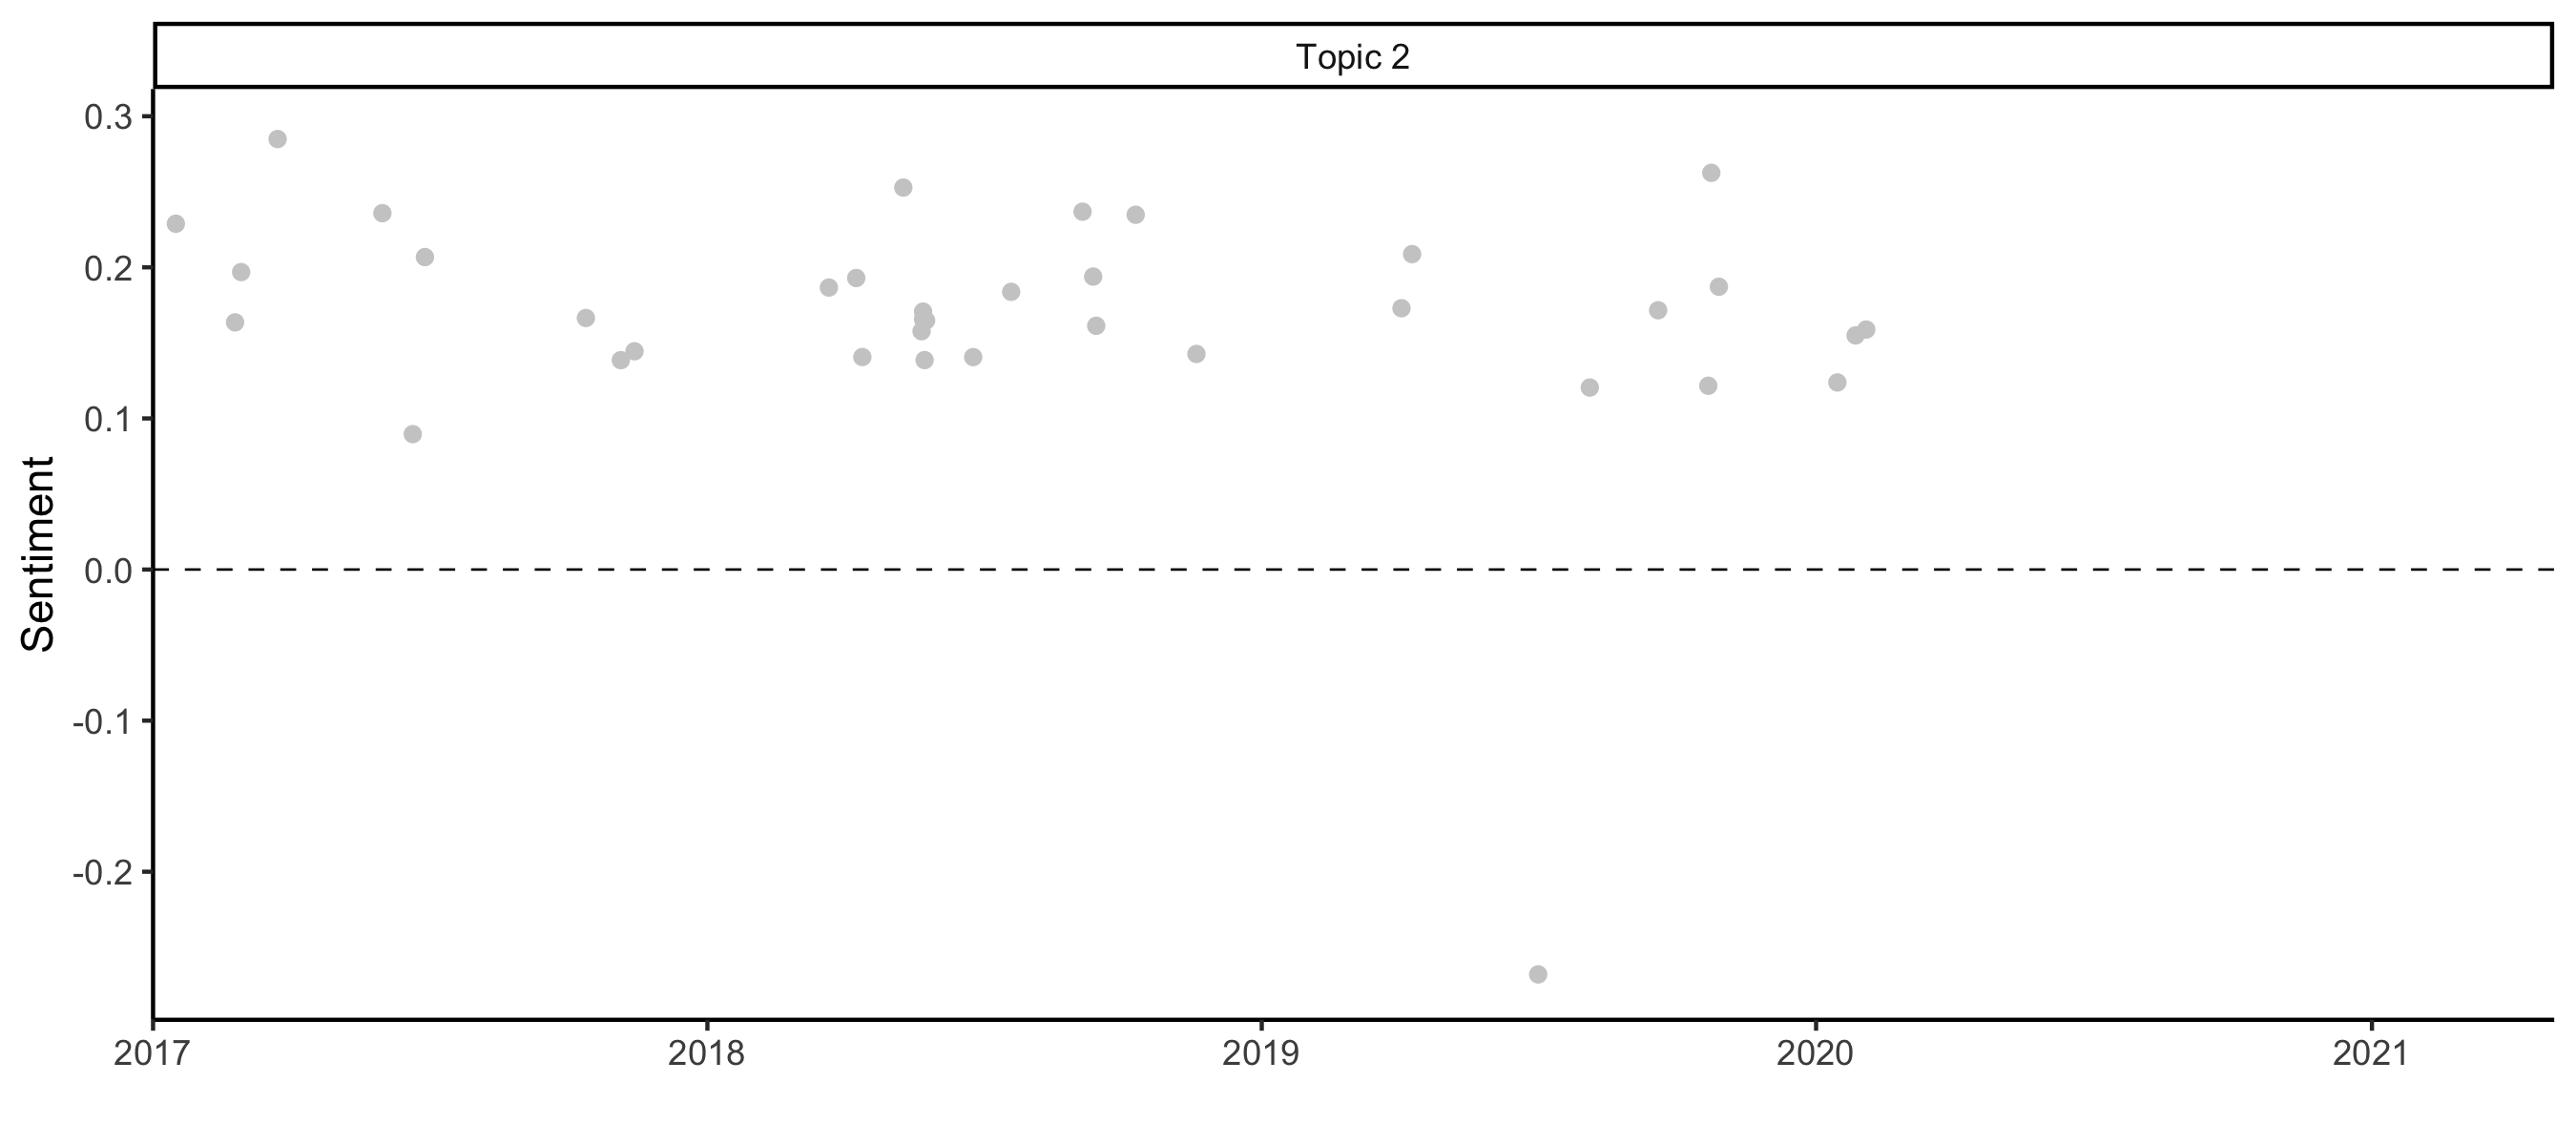
\includegraphics[width = \textwidth]{topic2red.png}
      }
   }
   \only<5-6>{
      \framesubtitle{Topic 3: Technology to fight the COVID-19 pandemic}
      \only<5>{
         \begin{figure}
            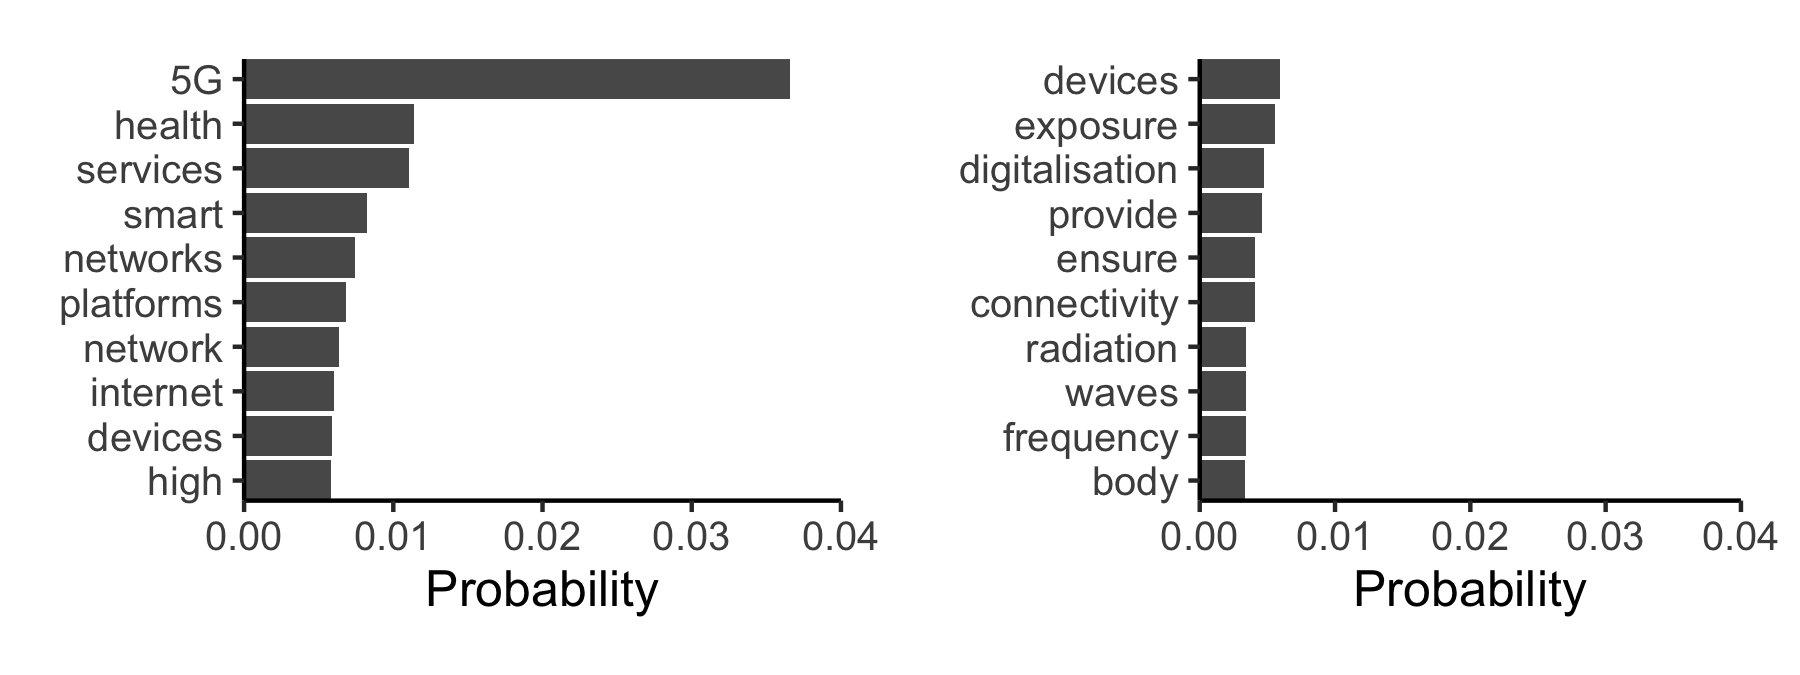
\includegraphics[width = \textwidth]{topic3.png}
            \caption{\alert{The left panel} shows the most probable words while \alert{the right panel} depicts probablity of the words that are unique only for the topic.}
         \end{figure}
      }
      \only<6>{
         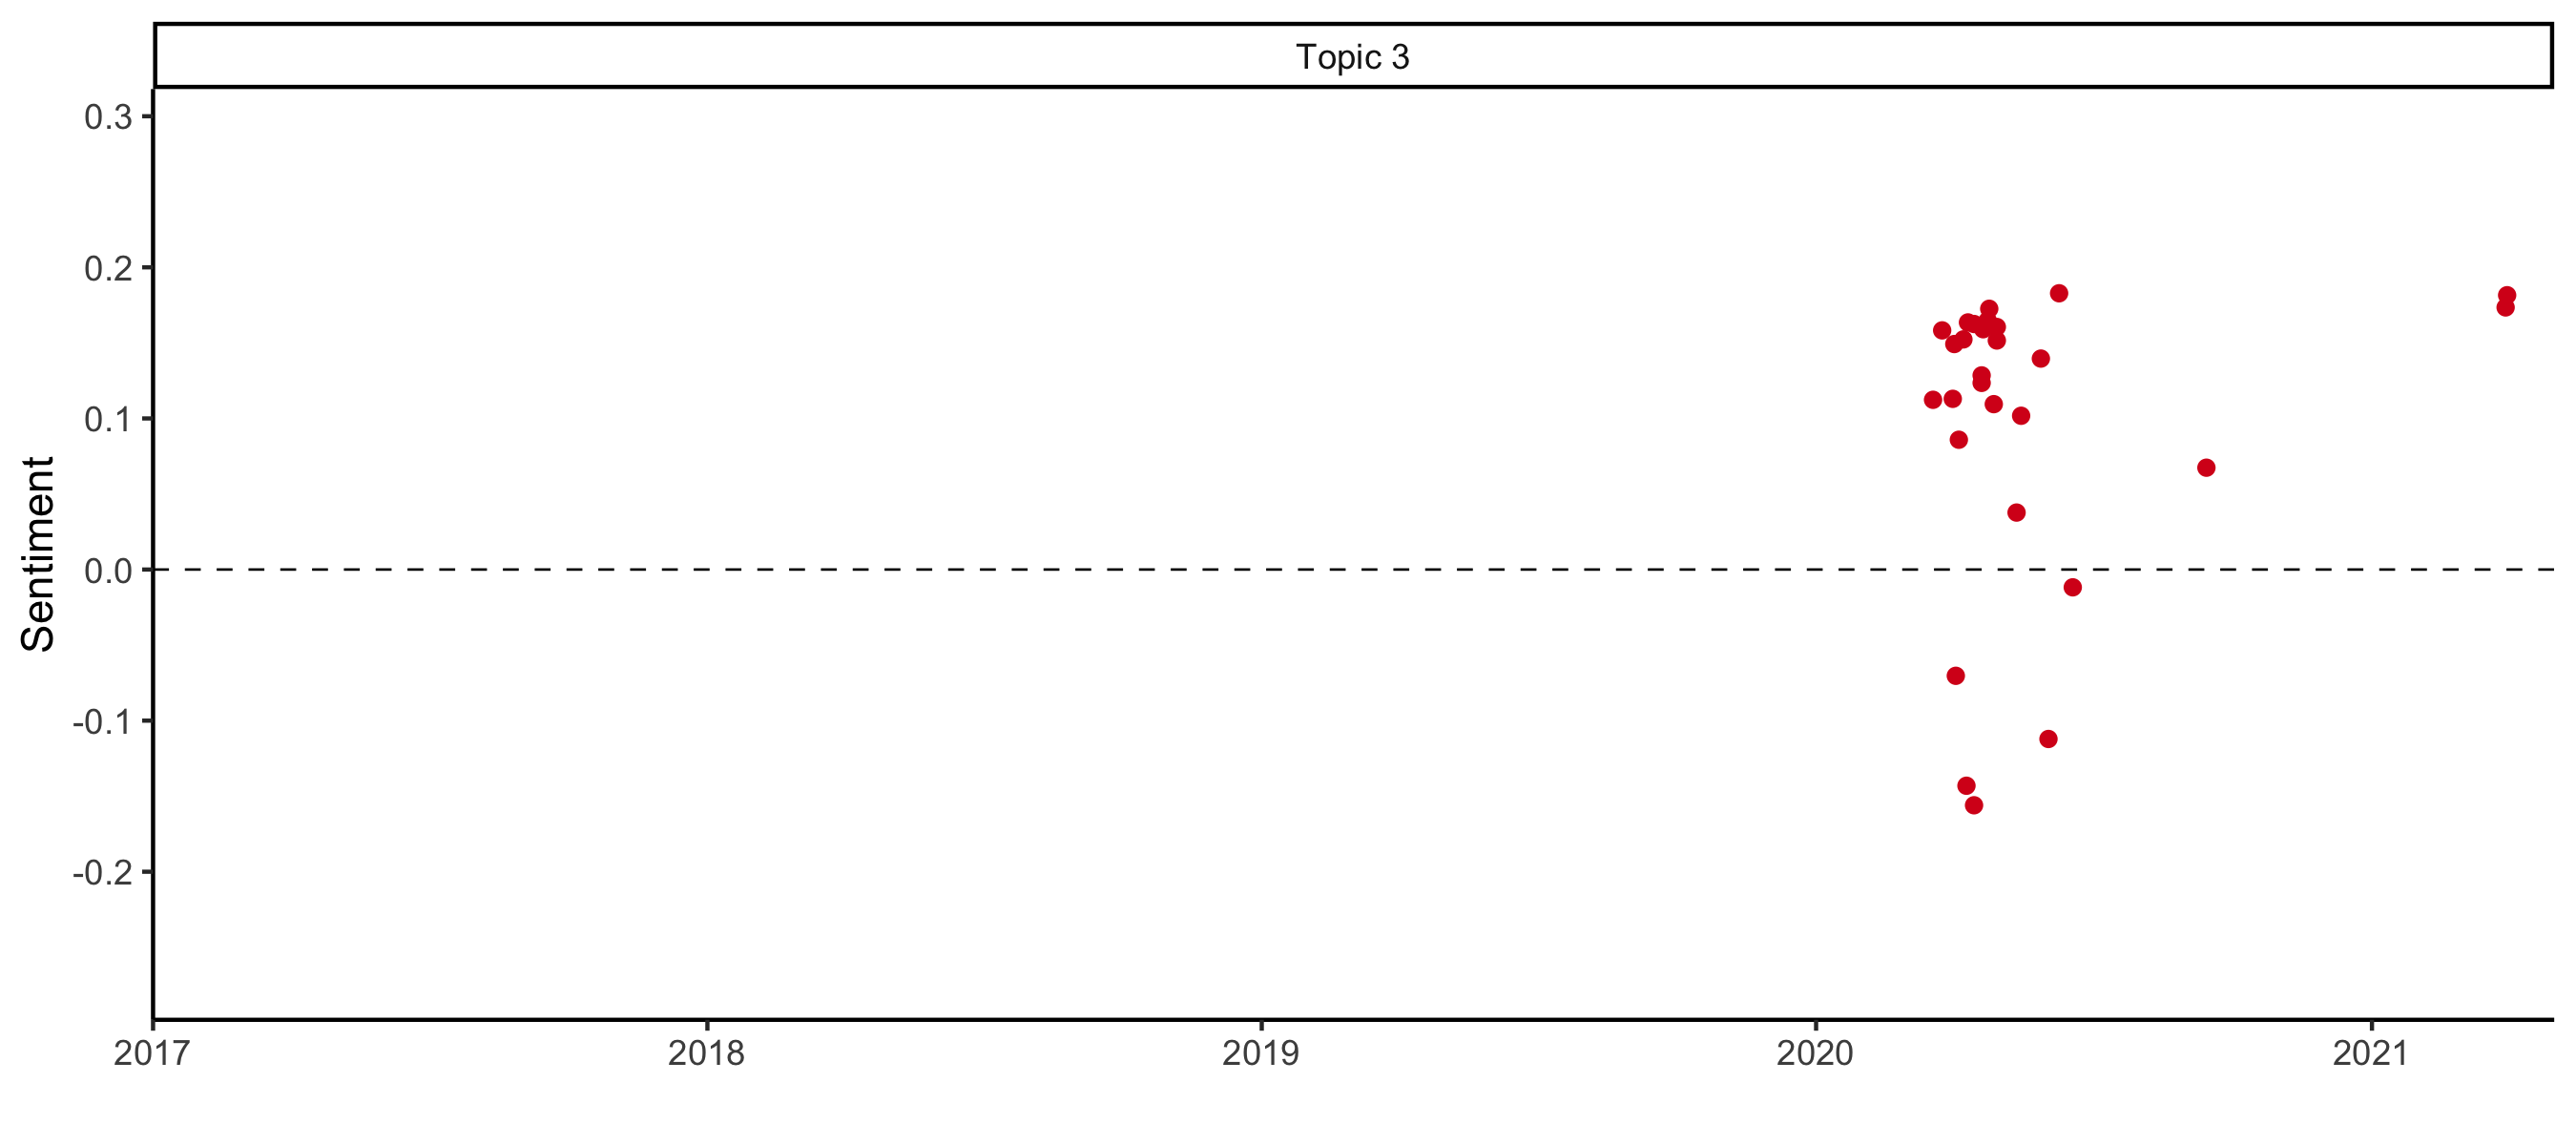
\includegraphics[width = \textwidth]{topic3red.png}
      }
   }
   \only<7-8>{
      \framesubtitle{Topic 4: For digitalisation of Europe}
      \only<7>{
         \begin{figure}
            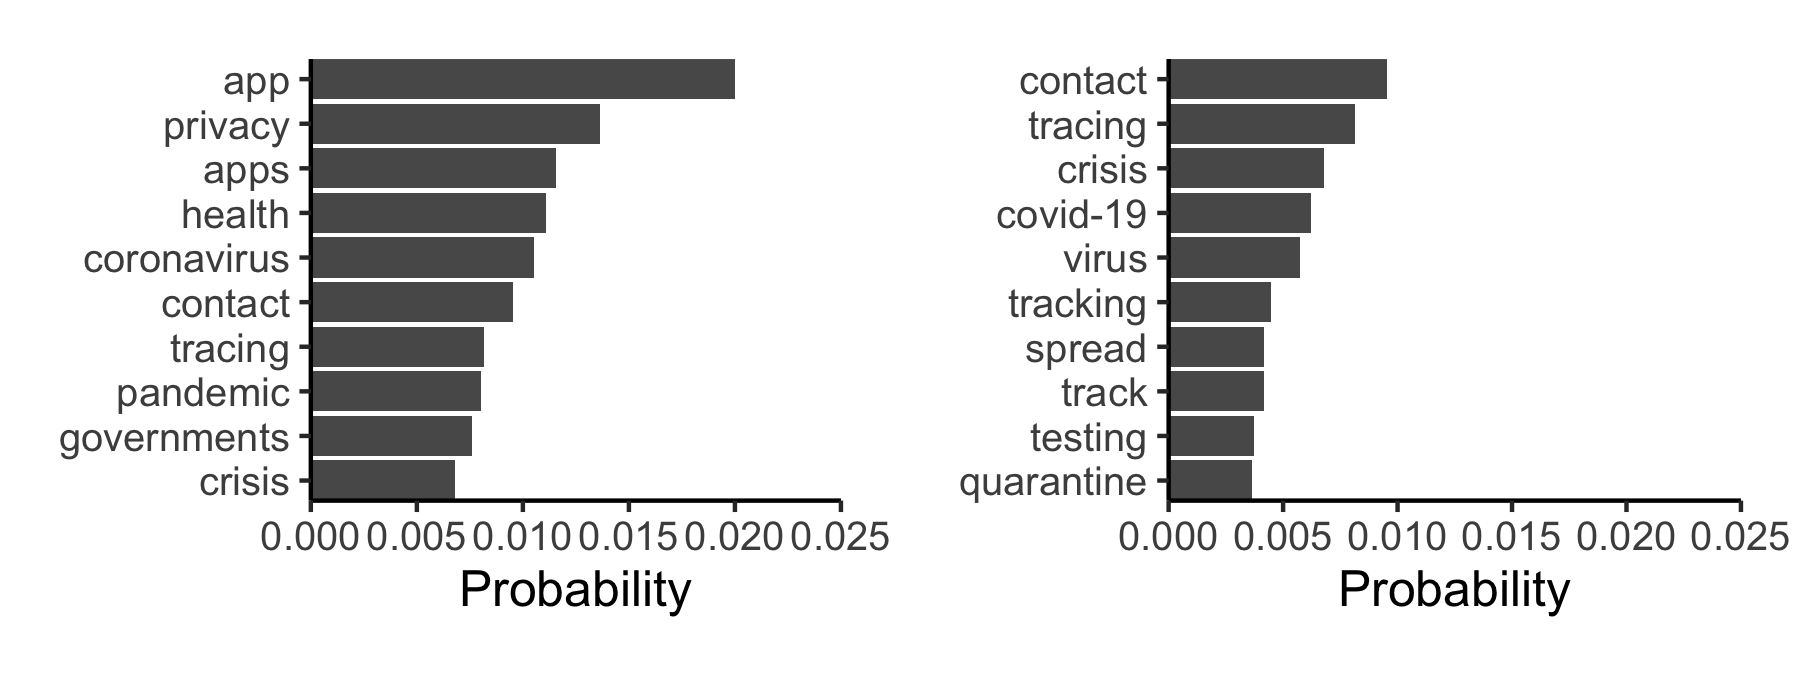
\includegraphics[width = \textwidth]{topic4.png}
            \caption{\alert{The left panel} shows the most probable words while \alert{the right panel} depicts probablity of the words that are unique only for the topic.}
         \end{figure}
      }
      \only<8>{
         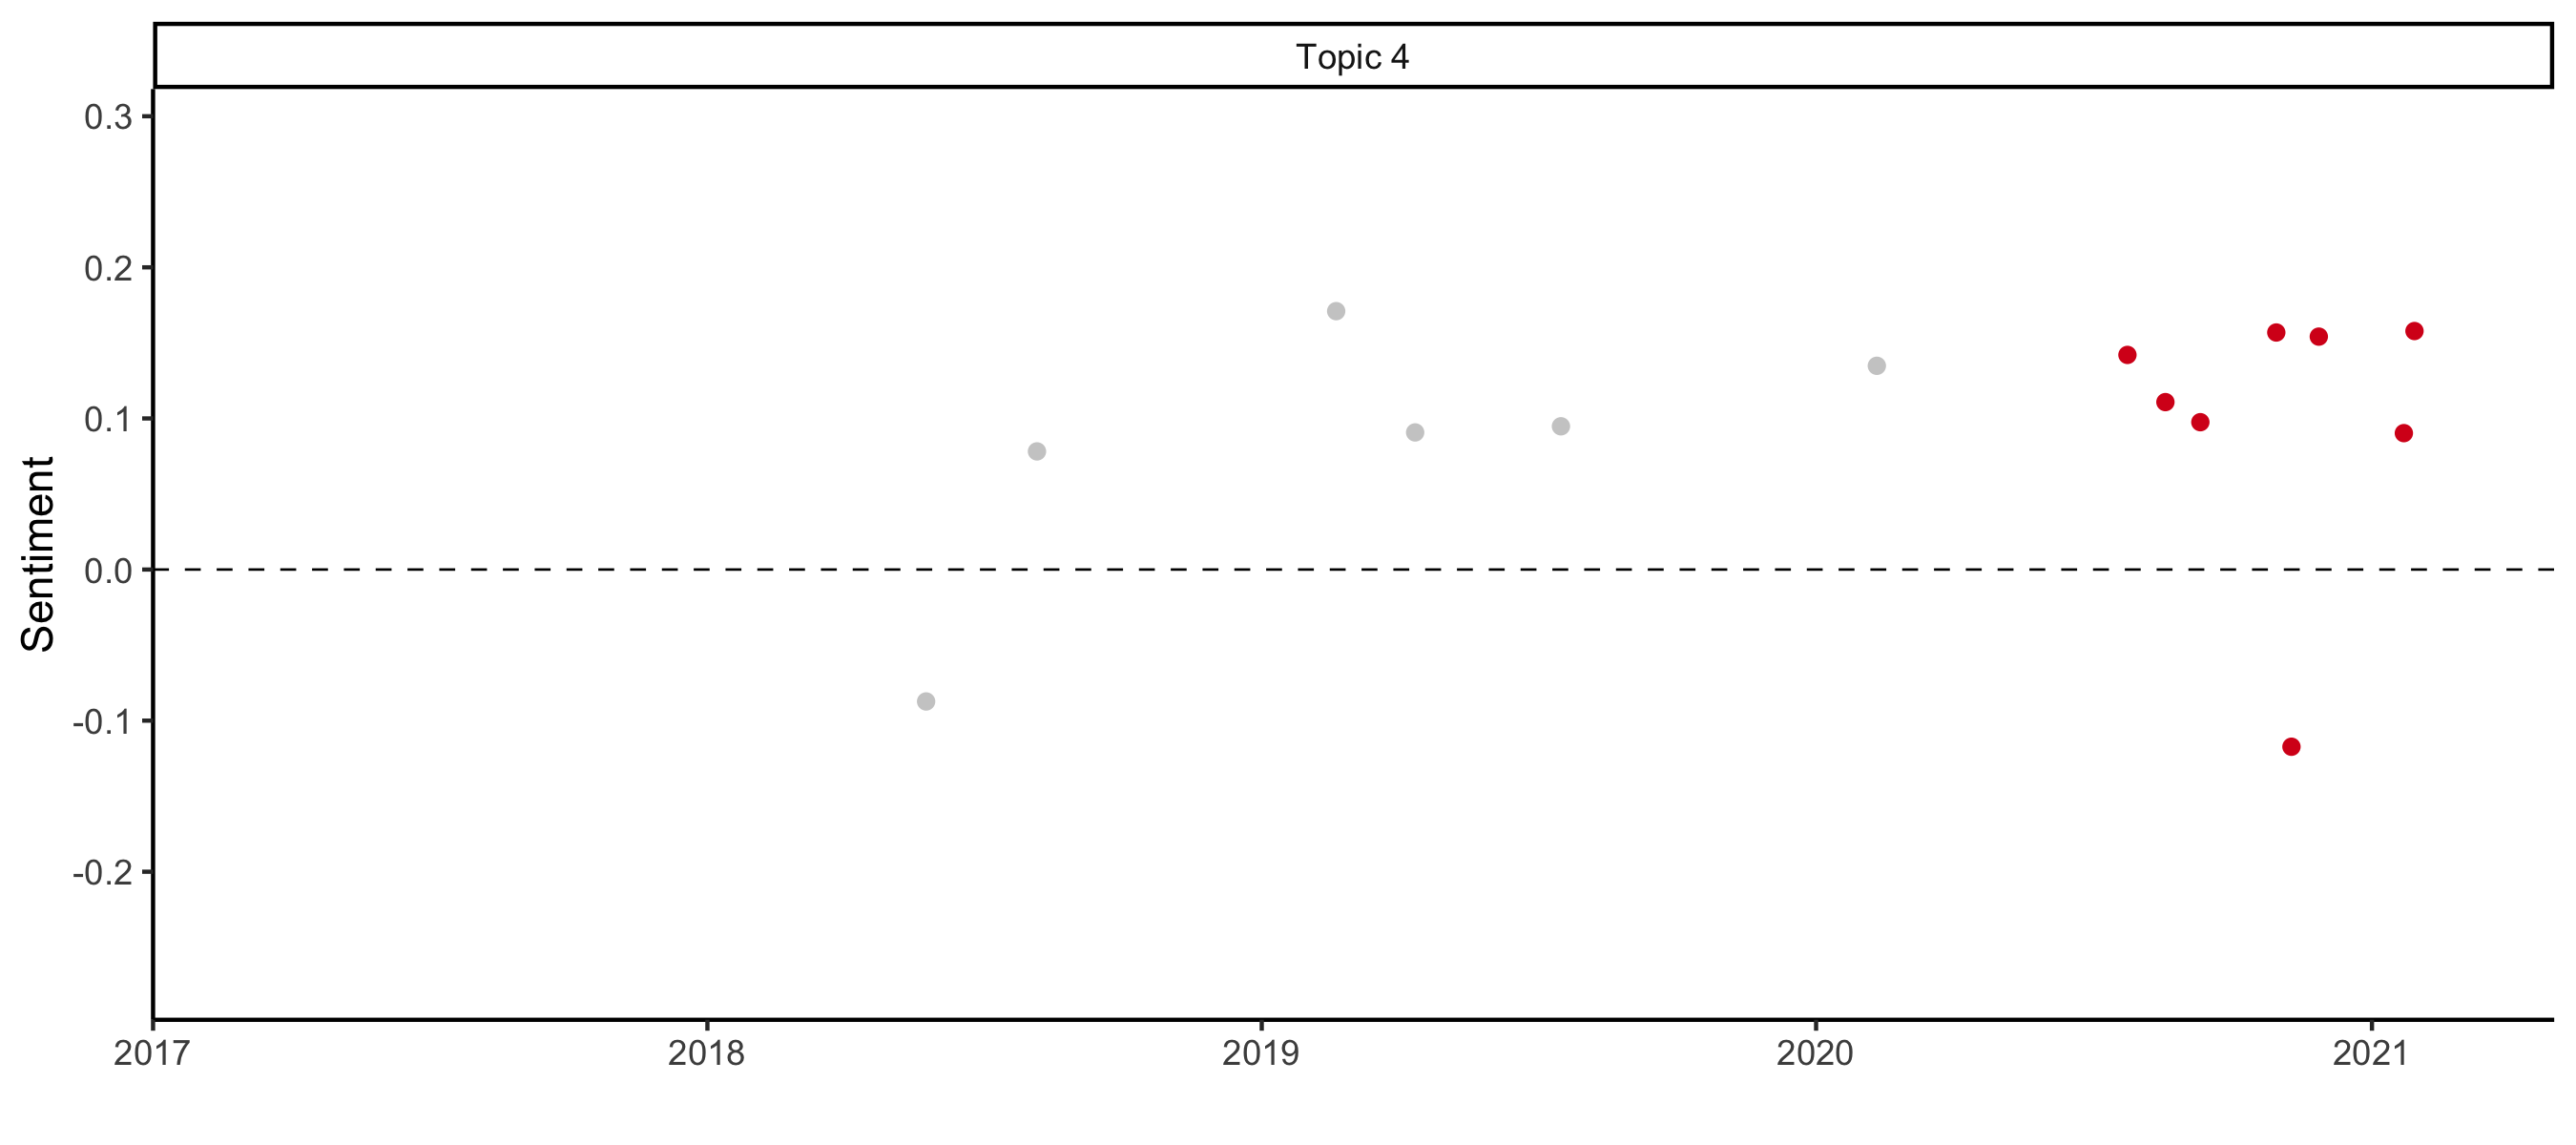
\includegraphics[width = \textwidth]{topic4red.png}
      }
   }
\end{frame}
\section{Qualitative Analysis}
\begin{frame}
   \frametitle{Qualitative Analysis}
   \only<1>{
      \framesubtitle{Perceived Sentiment Analysis}
      \centering
      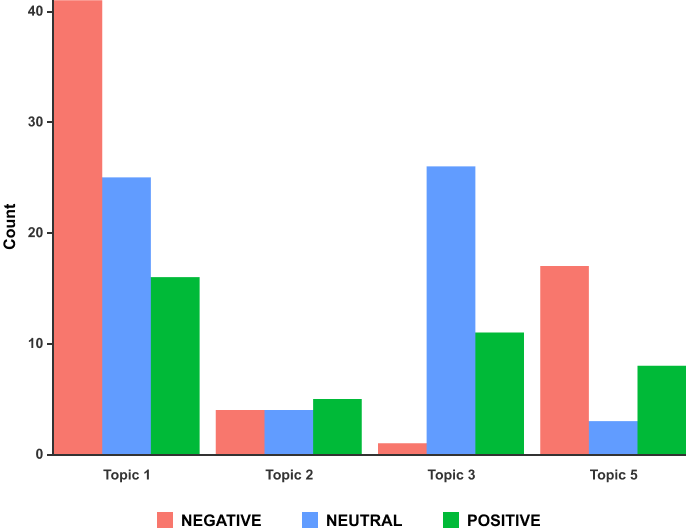
\includegraphics[width = .9\textwidth]{plot_sent.png}
   }
   \only<2-4>{
      \framesubtitle{Qualitative analysis of topics}
      \begin{itemize}
         \item<2-> Pandemic as a fast-tracking factor in technological development
         \item<3-> Privacy concerns
         \item<4> Trade-off between health and privacy
      \end{itemize}
         \only<2>{\begin{block}{}
            \blockquote[EUobserver, 2020-04-14]{%
               \small The resonse of EU countries to the coronavirus outbreak has prompted unprecedented levels of surveillance, data expoitation, and misinformation. Data collection can be essentail to understand and respond to the COVID-19 emergency, but creating such digital surveillance risks failure and adverse side-effect.%
            }
         \end{block}
         }
         \only<3>{\begin{block}{}
            \blockquote[POLITICO Europe, 2020-04-19]{%
               \small And almost 40 governments worldwide have rolled out -- or are about to -- their own coronavirus apps for everything from informing people if they've been in contact with anyone infected with COVID-19 to ensuring those that already have it stay home. All of this should set off alarm bells. Big Tech has become a global punching bag because of fears that Silicon Valley has too much control over our daily lives. But in their legitimate efforts to keep people safe, officials across the European Union, United States, and elsewhere are quickly falling into the same trap -- creating a government surveillance network on the fly, with little oversight and almost no clarity about when it will be shut down.%
            }
         \end{block}
         }
         \only<4>{
            \begin{block}{}
               \blockquote[Euronews Egnlish]{%
               Is there a trade-off to be had between privacy and public health? In these unprecedented times, there has been a monumental shift in personal liberties, and there is undoubtedly a trade-off to be had between privacy and the need to curtail the spread of the pandemic, but what measures are appropriate and will they have a long-lasting social effect? ''That's a million-dollar question,'' Woodhams said.%
               }
            \end{block}
         }

   }
%   \only<5>{
%      \framesubtitle{Main Actors}
%      \begin{itemize}
%         \small
%         \item Among \alert{cities were:} London (17), Berlin (14), Paris (11), and other cities like Hong Kong, Nice, Moscow, and Warsaw.
%         \item In terms of regions Europe (61) was the most cited but among \alert{countries} we had: Germany (79), China (79), USA (65), UK (58), France (52), Poland (23), Italy (15), Russia (14), Hungary (12), Switzerland (11), and Spain (10).
%         \item \alert{Tech Companies} were cited 353 times in the corpus, among the most mentioned we had: Google (66), Apple (56), and Facebook (29)
%         \item \alert{Euopean Union} institution was referred with the use of the following: EU (90), European Commission (14), and European Parliament (5)
%         \item Another highly visible group was \alert{Watchdog organizations}. With Amnesty International (6), Human Rights Watch (5), and Civil Liberties Union for Europe as the most cited.
%      \end{itemize}
%
%   }
   \only<5>{
      \framesubtitle{Main Technologies}
      \begin{itemize}
         \small
         \item \alert{Tracing apps} were usually mentioned in the newest set of articles related to the COVID-19 pandemic and usually described as ''necessary evil''.
         \item \alert{Facial Recognnition} and \alert{Artificial Intelligence} are often mentioned in the context of privacy concerns and police efforts to introduce safety measures in the public spaces. Some articles point out \alert{bias and serious threats of discrimination of specific social groups}.
         \item The tone of the narrative on \alert{5G} changes over time, from warnings against the dominance of non-European suppliers to potential behind the 5G to boost digitalization of Europe.
         \item The technological development was also linked with \alert{envioronmental goals and challenges} such as \alert{climate emergency}.
      \end{itemize}
   }
   \only<6-8>{
      \small
      \framesubtitle{Technology threats}
      \begin{itemize}
         \item<6-> Existing abuse of technologies by authoritarian regimes as a ''dark scenario''
         \item<7-> Potential abuse of technologies by European governments and police -- the creation of high-tech surveillance state or surveillance cities, government distrust
         \item<8> Strengthening prejudice and discrimination though biased AI
      \end{itemize}
      \only<6>{
         \begin{block}{}
            \blockquote[POLITICO Europe, 2019-06-24]{%
               The emerging technologies can, for example, be abused by authoritarian regimes to set up a ubiquitous surveillance apparatus. Most prominently, China has been using cutting-edge AI to build up a high-tech surveillance system and a crackdown on political dissent, according to media reports – and other countries around the world, including European nations such as Serbia, have struck deals with Chinese companies to introduce their own systems aimed at monitoring individuals.%
            }
         \end{block}
      }
      \only<7>{
         \begin{block}{}
            \blockquote[POLITICO Europe, 2020-01-24]{%
            Democratic governments in the West are increasingly following the example of authoritarian regimes in deploying the technology, which allows them to scan faces in crowds, compare the results with stored data and identify individuals in real-time. Civil rights advocates have warned that such ”live” or ”automated” facial recognition systems pave the way for mass surveillance on an unprecedented scale (...).%
            }
         \end{block}
      }
      \only<8>{
         \begin{block}{}
            \blockquote[POLITICO Europe, 2020-09-06]{%
            Most of today’s cutting-edge AI systems are, for example, prone to discriminate against vulnerable groups and minorities. This has led to text analysis software labeling being Jewish or being gay as negative, British students from poor areas being disadvantaged during exams, or a Black American being arrested for a crime he did not commit.%
            }
         \end{block}
      }
   }
\end{frame}
\section{Summary}
\begin{frame}
   \frametitle{Summary}
   \only<1>{
      \begin{enumerate}
         \item Mixed-methods approach allows for a more accurate evaluation of the sentiment than algorithm-based analysis.
         \item Topic Modeling algorithms (LDA) seem to be accurate enough for reviewing a large corpus of texts.
         \item Call for an open and inclusive public conversation about smart city development and surveillance implementations.
         \item Europe needs to step up its game to avoid marginalization or even takeover by global tech players in ''digital race''.
         \item Arguments around technology are centered around economical interest rather than citizens’ rights and concerns.
      \end{enumerate}
   }
   \only<2>{
      \frametitle{Thank You!}
      \begin{block}{}
         \blockquote[EURACTIV, 2021-09-02]{%
            (...) the EU and its member states need to provide adequate funding for key technologies such as AI, blockchain, the Internet of Things, and high-performance computing now during these difficult times of tacking the pandemic. This is the only way we can meet our European environmental and climate goals, enable inclusively, socially just, and sustainable economic growth, and ensure an increase in competitiveness and prosperity.%
         }
      \end{block}
   }
\end{frame}

\part[Projects]{Projects}
\frame{\partpage}

\section[Forms of the project]{Forms of the project}
\begin{frame}{Possible forms of the project}
    \begin{enumerate}
     \item \textbf{Research project proposal.} A short proposal for a research
     project using some of the methods we discussed in the class. Details are
     discussed in \textit{Structure of the proposal} section.
     \item \textbf{Simple research project and report.} Simple data-driven
     project in which you gather some data from an external web-based source
     (i.e. from an API or through webscraping), process it and use it to answer
     a simple research question. Details are discussed in \textit{Structure of
     the project} section.
    \end{enumerate}
\end{frame}
    
\section[Structure of the project]{Structure of the project}
\begin{frame}{Structure of the proposal | general information}
    \begin{itemize}
     \item \textbf{Introduction and problem statement.} This section should
     explain what is the project about in general and why the given problem
     matters. The significance of the problem may be justified both in terms of
     its theoretical/scientific or societal/business relevance.
     \item \textbf{Research question.} What is the specific research question
     you will try to answer in the project? It can be either formulated as a
     strict hypothesis or as an exploratory question (i.e. not assuming any
     particular effect or mechanism).
     \item \textbf{Research methods.} This section should discuss, at a general
     level, what data do you plan to use and how will analyze it. In particular,
     you should clearly explain why the data and methods you chose will allow
     you to answer your research question.
    \end{itemize}
\end{frame}
    
\begin{frame}{Structure of the proposal | research methods}
    \begin{itemize}
     \item \textbf{Data collection.} What is the data you are planning to use?
     Where is it stored and how do you plan to obtain/extract it?  Are there any
     possible obstacles and if there are what can be done to minimize the risk
     of failure?
     \item \textbf{Data preprocessing and storage.} How will you preprocess data
     and in what format will store it for later use? For instance, when scraping
     you may decide to data gathered from every individual website to a JSON
     object and store all data in \texttt{.jl} file (JSON lines).
     \item \textbf{Analytic methods.} What analytic methods will you apply to
     your data in order to answer your question? This may include some methods
     that we discussed in the class (i.e. sentiment analysis or some other
     natural language processing methods), but you should also use your general
     statistical knowledge to decide how you want to model your final data.
    \end{itemize}
\end{frame}
    
\begin{frame}{Structure of the project | general methods}
    \begin{itemize}
     \item The project should consist of two main items:
     \begin{enumerate}
     \item \textbf{Notebook} with code and description of the project.
     More on that below.
     \item File with the \textbf{raw data} as was extracted from the external
     data source (e.g. API or webpage).
     \end{enumerate}
     \item The notebook should include a short introduction describing the
     problem and why it is significant.
     \item The specific research question should be introduced.
     \item Data source should be discussed. In particular in relation to the
     research question.
     \item Data analysis methods should be discussed, also in relation to the
     research question.
     \item Code and text should be mixed in the notebook in a way that
     facilitates understanding of the adopted research methods and obtained
     results.
    \end{itemize}
\end{frame}
    
\section[Things to remember]{Things to remember}
\begin{frame}{Things to remember}
    \begin{itemize}
     \item Make sure you will be able to gather data legally.  For instance, if
     you want to scrape some websites you should try to determine whether they
     allow scraping. You can check this by looking at the so-called
     \texttt{robots.txt} of a website.  It can be found at
     \texttt{<url>/robots.txt}. For instance, you can see Facebook configuration
     at \texttt{facebook.com/robots.txt}.
     \item Be kind for your data source. If there is a platform that exposes an
     API you should use it instead of scraping data directly from its webpage.
     \item Think about proper format for storing data. If you plan to use your
     data to compute a statistical model in SPSS may be JSON lines are not the
     best and you should consider storing your data as a simple CSV file?
    \end{itemize}
\end{frame}
    
\section[Formal requirements]{Formal requirements}
\begin{frame}
        \frametitle{Formal requirements}
        \only<1>{
            \begin{itemize}
            \item Regardless whether you chose a project or a proposal the
            deadline for submitting it is on \textbf{XX.XX.2023 23:59:59}.
            \item If you decide to submit a project please send us two files:
            the notebook and the raw data file. Please, remember to rename them
            properly FP\_<SURNAME>\_<NAME>.ipynb and FP\_<SURNAME>\_<NAME>.jl
            (the data file might have the format of your choice, it doesn't have
            to be a JSON line file).
            \item If you decide to submit a proposal your work should not be
            shorter than 3 pages and not longer than 5 (interline: single, font
            size: 12). Please, remember to rename your file properly
            FP\_<SURNAME>\_<NAME>.docx.
            \item Regardless whether you will choose proposal or project you
            must include at least one bibliography item.
            \end{itemize}
        }
        \only<2>{
            \begin{block}{}
                Last but not least, it must look aesthetically. Please, spend
                some time on formatting and checking spelling and grammar.
            \end{block}
        }
    \end{frame}


\end{document}